\newsection{Processor VS CPU VS Core}
\index{Processor}
\index{CPU}
\index{Core}
\begin{itemize}
    \item \textbf{Processor} is a~general name of~any gadget that can read instructions and~perform actions according to~these instructions (i.e.,~that can process instructions).
    \item \textbf{CPU} (Central Processing Unit) is a~specific type of~processor. It's the main processor in a~computer controlling the~behavior of~all other parts of the~computer. Nowadays CPU is treated as a~synonym of the~processor, but that's wrong. Beside the~CPU there are~other processors in a~computer. For~example, a~hard drive contains its own processor controlling data reading and~writing, graphic cards contain a~GPU (Graphics Processing Unit) performing calculations needed to render and~display images etc.
    \item \textbf{Core} is the main computation component of the CPU performing instructions (with the~help of~other parts of the~core like \hyperref[alu]{ALUs}). Typically, one core can process one instruction at~a~time, although nowadays there are even cores enabling parallel instructions processing. However, standardly the~parallelism is still achieved by putting more cores to one CPU and~more CPUs to~one computer. For~example, when you read the~typical "state--of--the--art" claim that a~computer has~quad--core processor, it means that there is a~single CPU with four cores in the~computer. Beside cores CPUs also contain switch bridges (distributing instructions to~cores), caches and~other stuff.
\end{itemize}

\newsection{32b VS 64b}
\index{32b}
\index{64b}
\label{32bvs64b}

\newsection{ALU}
\index{ALU}
\index{Arithmetic logic unit}
\index{Logic gate}
\label{alu}
The~abbreviation stands for~\textit{Arithmetic Logic Unit}. It's an electronic circuit that performs arithmetic and~bitwise operations on~integer binary numbers.

\newline\warning Do not confuse it with a~simple electronic device performing a~boolean operation over two bits (AND, OR, XOR etc.). That's called \textit{Logic Gate}. An~ALU consists of multiple logic gates.

\newline\warning ALUs are parts of~CPUs, but not cores. A~core is connected with an~ALU via an~execution port, sends inputs to it and processes returned results.

\begin{figure}
    \centering
    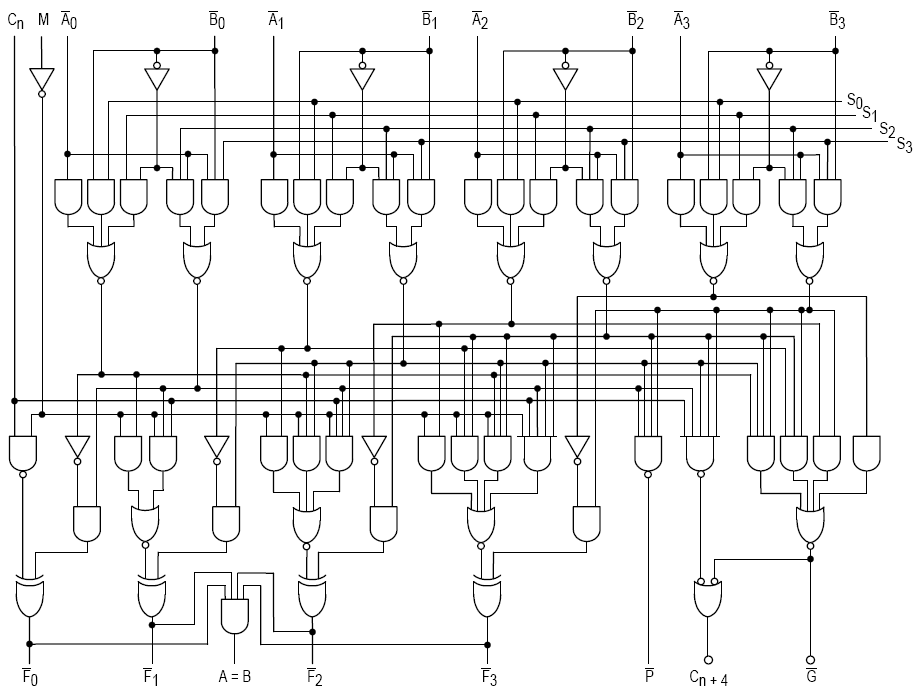
\includegraphics[width=\textwidth]{pictures/ALU.png}
    \caption*{An example of a simple (no joke) four--bit ALU}
\end{figure}